\chapter{OpenMP}
%\label{chapter:title}

In this assignment the heat code was parallelized using OpenMP pragmas. Then, process distribution in the architecture was optimized using the environment variable \verb|KMP_AFFINITY|.

% \section*{4.1 Sequential performance}
% Test the provided optimized code version available in Moodle. Report the initial performance for all test configuration in test.dat. Run in batch. We want to make sure that all of you have the same base performance. Do not change the compiler flags. 


% \section*{4.2 Automatic parallelization}
% Provide a speedup graph for the given configurations where the x-axis is the number of threads and the y-axis the achieved speedup. Use the reported execution time for the sequential code (Assignment 4.1) as the basis for the speedup calculation

\section*{Parallelization of the code}
% Provide a speedup graph comparing with and without first touch for the two configurations (2000,6000). Without any special Affinity settings. 
% Provide a speedup graph for the configurations (2000, 6000) with two curves for cyclic and block thread distribution with first touch. 
% Run also measurements with vtune for your best OpenMP version with 3200 resolution. Compare the measurements to the vtune results with a single thread. Submit interesting graphs with annotations.

The parallelization was done on the loops accessing the main array, specifically the for loops inside the 
 \verb|relax_jacobi| function and the \verb|initialize| function. The directives used for the loop in the \verb|initialize| function were \verb|omp for|, while for the loop inside \verb|relax_jacobi| also \verb|reduction(+:sum)| was added. The reduction allows to have a private variable \verb|sum| for each process and aggregate each one at the end.

The parallelization of the initialisation loop is particularly important because it takes into account NUMA's first touch policy: the data page is allocated in the memory closest to the thread accessing this page for the first time. This allows a better memory distribution and therefore speedup compared to a sequential code, as can be seen in Figure \ref{fig:first-touch}. 
The miss rate is the ratio between cache misses and the sum of cache hits and misses, both obtained by LIKWID measurements.

\begin{figure}[h]
    \centering
    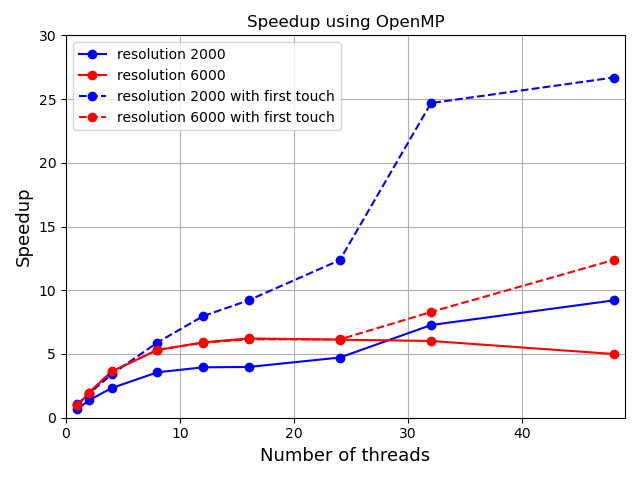
\includegraphics[width=0.7\linewidth]{figures/first_touch.png}
    \caption{Comparison of the runtime speed up (with respect to the sequential code) for heat code with and without parallelization of the initialization.}
    \label{fig:first-touch}
\end{figure}

Figure \ref{fig:first-touch} also displays a drop in the speedup trend at 24 threads. This suggests there is a shift between the use of only one socket at 24 threads and both sockets after 24 threads. The full use of the socket can cause higher competition for the communication bandwidth within the socket.


\section*{Thread Affinity Interface}
The Intel runtime library can bind OpenMP threads to physical processing units and specifically restrict the execution of the threads to a certain set of physical processing units, which can lower the runtime.

This can be done through the the environment variable \verb|KMP_AFFINITY|, and its attributes. With the attribute \verb|type| it is possible to set the affinity type: \verb|scatter| distributes the threads as evenly as possible across the entire system, \verb|compact| is its opposite and it places the current threads next to the previous thread. Other options in between are also available. 
%thread context: all the information the thread needs to seamlessly resume execution, including the thread's set of CPU registers and stack.

The two affinities \verb|compact| and \verb|scatter| were compared in Figure \ref{fig:kmp-affinity}, which shows a clear advantage of the scatter affinity especially for the lower resolution. This could be due to the fact that there is less bus contention between the threads, and would also explain the reduction in speedup when the thread number increases. 


\begin{figure}[h]
    \centering
    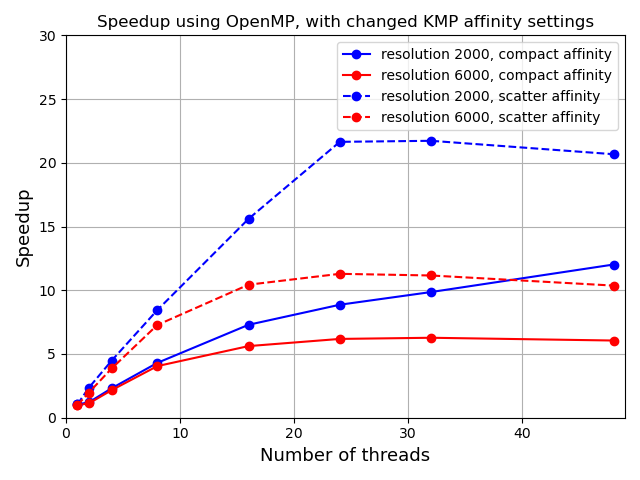
\includegraphics[width=0.7\linewidth]{figures/kmp_affinity.png}
    \caption{Comparison of the runtime speed up (with respect to the sequential code) for heat code with compact and scatter affinity type.}
    \label{fig:kmp-affinity}
\end{figure}

Through the attribute \verb|modifier| it is possible to set the granularity, which describes the lowest level that a thread can float in. This is useful for runtime, because binding threads to a specific thread context is not necessarily beneficial. In this case the best performing granularity was \verb|fine|, which binds each thread to a single thread context.

% The default configuration for KMP affinity, shown in Figure \ref{fig:first-touch}, does not bind the OpenMP threads, and has as better performance for higher numbers of threads. (!!)
